\section{Algoritmo di Hoshen-Kopelman}
L’algoritmo di Hoshen-Kopelman (HK76) rappresenta una tecnica di etichettatura dei cluster. Il reticolo viene visitato sito per sito per colonne, partendo dallo spigolo in alto a sinistra per arrivare a quello in basso a destra. Si prenda, ad esempio, il reticolo in Figura \ref{fig:basegrid}
\begin{figure}[H]
	\centering
	\scriptsize % Riduce la dimensione del testo
	\setlength{\tabcolsep}{5.4pt} % Riduce lo spazio tra le colonne
	\renewcommand{\arraystretch}{1.2} % Riduce lo spazio verticale tra le righe
	\begin{minipage}{0.4\textwidth}
		\centering
		\begin{tabular}{|*{15}{c|}}
			\hline
			0 & 1 & 0 & 0 & 1 & 1 & 0 & 0 & 0 & 1 & 0 & 1 & 0 & 1 & 0 \\
			\hline
			0 & 1 & 1 & 0 & 0 & 0 & 1 & 0 & 0 & 1 & 1 & 1 & 1 & 1 & 1 \\
			\hline
			0 & 1 & 0 & 0 & 0 & 1 & 1 & 1 & 1 & 0 & 0 & 1 & 0 & 0 & 0 \\
			\hline
			1 & 0 & 1 & 0 & 1 & 0 & 1 & 0 & 0 & 0 & 1 & 1 & 0 & 0 & 0 \\
			\hline
			0 & 1 & 0 & 1 & 1 & 0 & 1 & 0 & 0 & 0 & 1 & 0 & 0 & 1 & 0 \\
			\hline
			0 & 0 & 1 & 1 & 1 & 1 & 1 & 0 & 1 & 1 & 1 & 1 & 1 & 0 & 1 \\
			\hline
			0 & 0 & 1 & 1 & 1 & 0 & 0 & 0 & 0 & 1 & 1 & 1 & 1 & 0 & 1 \\
			\hline
			0 & 1 & 0 & 1 & 1 & 1 & 1 & 0 & 1 & 1 & 1 & 1 & 0 & 1 & 0 \\
			\hline
			0 & 1 & 0 & 0 & 1 & 1 & 0 & 0 & 1 & 1 & 1 & 1 & 0 & 0 & 1 \\
			\hline
			1 & 0 & 0 & 0 & 0 & 0 & 0 & 0 & 1 & 0 & 0 & 0 & 0 & 1 & 0 \\
			\hline
			0 & 0 & 0 & 0 & 1 & 0 & 1 & 0 & 1 & 1 & 0 & 1 & 1 & 1 & 1 \\
			\hline
			1 & 1 & 0 & 0 & 0 & 1 & 0 & 1 & 0 & 1 & 1 & 1 & 1 & 1 & 1 \\
			\hline
			1 & 1 & 1 & 0 & 0 & 1 & 1 & 0 & 1 & 0 & 0 & 1 & 0 & 0 & 0 \\
			\hline
			0 & 1 & 0 & 1 & 1 & 1 & 1 & 1 & 0 & 1 & 1 & 1 & 0 & 1 & 1 \\
			\hline
			1 & 1 & 1 & 1 & 0 & 0 & 0 & 0 & 1 & 1 & 1 & 1 & 1 & 1 & 0 \\
			\hline
		\end{tabular}
	\end{minipage}
	\hfill
	\begin{minipage}{0.44\textwidth}
		\centering
		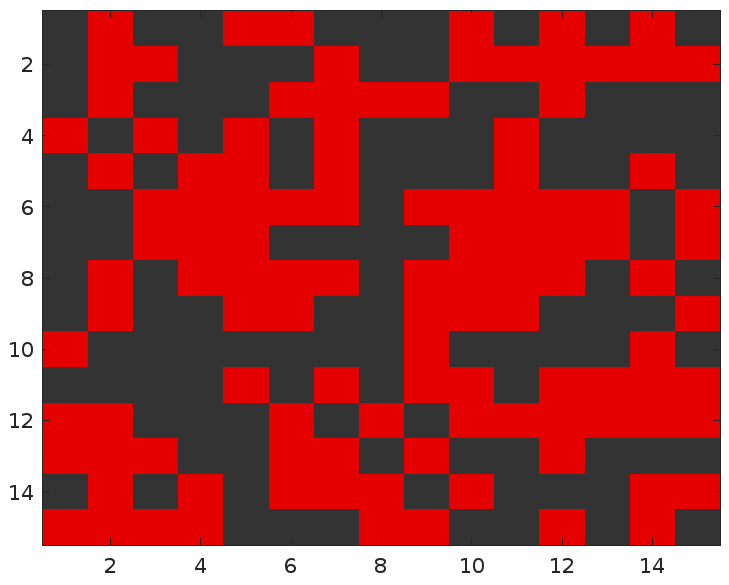
\includegraphics[width=\linewidth]{images/basegrid}
	\end{minipage}
	\label{fig:basegrid}
	\caption{Esempio di reticolo quadrato $15 \times 15$ con siti colorati (\textit{rossi}) e non colorati (\textit{neri})}
\end{figure}
\noindent
Durante la visita del reticolo, quando si incontra un sito colorato, allora: \textbf{(1)} Se il sito non è connesso ad altri siti colorati sopra o a sinistra, si inizia un nuovo cluster, a cui viene assegnata una \texttt{label} \textbf{(2)} Se c’è un primo vicino sopra o a sinistra colorato (ma uno solo dei due), il sito viene aggiunto al cluster del primo vicino colorato \textbf{(3)} Se i suoi primi vicini sono entrambi colorati, \textit{ma appartengono allo stesso cluster}, il sito viene aggiunto al cluster dei primi vicini \textbf{(4)} Se i suoi primi vicini sono entrambi colorati, e \textit{non appartengono allo stesso cluster}, il sito viene aggiunto al cluster con la \texttt{label} minore. 
\begin{figure}[H]
	\centering
	\scriptsize % Riduce la dimensione del testo
	\setlength{\tabcolsep}{3.5pt} % Riduce lo spazio tra le colonne
	\renewcommand{\arraystretch}{1.2} % Riduce lo spazio verticale tra le righe
	\begin{minipage}{0.3\textwidth}
		\centering
		\begin{center}
			\begin{tabular}{|*{15}{c|}}
				\hline
				0 & 1 & 0 & 0 & 2 & 2 & 0 & 0 & 0 & 3 & 0 & 4 & 0 & 5 & 0 \\
				\hline
				0 & 1 & 1 & 0 & 0 & 0 & 6 & 0 & 0 & 3 & 3 & 3 & 3 & 3 & 3 \\
				\hline
				0 & 1 & 0 & 0 & 0 & 7 & 6 & 6 & 6 & 0 & 0 & 3 & 0 & 0 & 0 \\
				\hline
				8 & 0 & 9 & 0 & 10 & 0 & 6 & 0 & 0 & 0 & 11 & 3 & 0 & 0 & 0 \\
				\hline
				0 & 12 & 0 & 13 & 10 & 0 & 6 & 0 & 0 & 0 & 11 & 0 & 0 & 14 & 0 \\
				\hline
				0 & 0 & 15 & 13 & 10 & 10 & 6 & 0 & 16 & 16 & 11 & 11 & 11 & 0 & 17 \\
				\hline
				0 & 0 & 15 & 13 & 10 & 0 & 0 & 0 & 0 & 16 & 11 & 11 & 11 & 0 & 17 \\
				\hline
				0 & 18 & 0 & 13 & 10 & 10 & 10 & 0 & 19 & 16 & 11 & 11 & 0 & 20 & 0 \\
				\hline
				0 & 18 & 0 & 0 & 10 & 10 & 0 & 0 & 19 & 16 & 11 & 11 & 0 & 0 & 21 \\
				\hline
				22 & 0 & 0 & 0 & 0 & 0 & 0 & 0 & 19 & 0 & 0 & 0 & 0 & 23 & 0 \\
				\hline
				0 & 0 & 0 & 0 & 24 & 0 & 25 & 0 & 19 & 19 & 0 & 26 & 26 & 23 & 23 \\
				\hline
				27 & 27 & 0 & 0 & 0 & 28 & 0 & 29 & 0 & 19 & 19 & 19 & 19 & 19 & 19 \\
				\hline
				27 & 27 & 27 & 0 & 0 & 28 & 28 & 0 & 30 & 0 & 0 & 19 & 0 & 0 & 0 \\
				\hline
				0 & 27 & 0 & 31 & 31 & 28 & 28 & 28 & 0 & 32 & 32 & 19 & 0 & 33 & 33 \\
				\hline
				34 & 27 & 27 & 27 & 0 & 0 & 0 & 0 & 35 & 32 & 32 & 19 & 19 & 19 & 0 \\
				\hline
			\end{tabular}
		\end{center}
	\end{minipage}
	\hfill
	\begin{minipage}{0.45\textwidth}
		\centering
		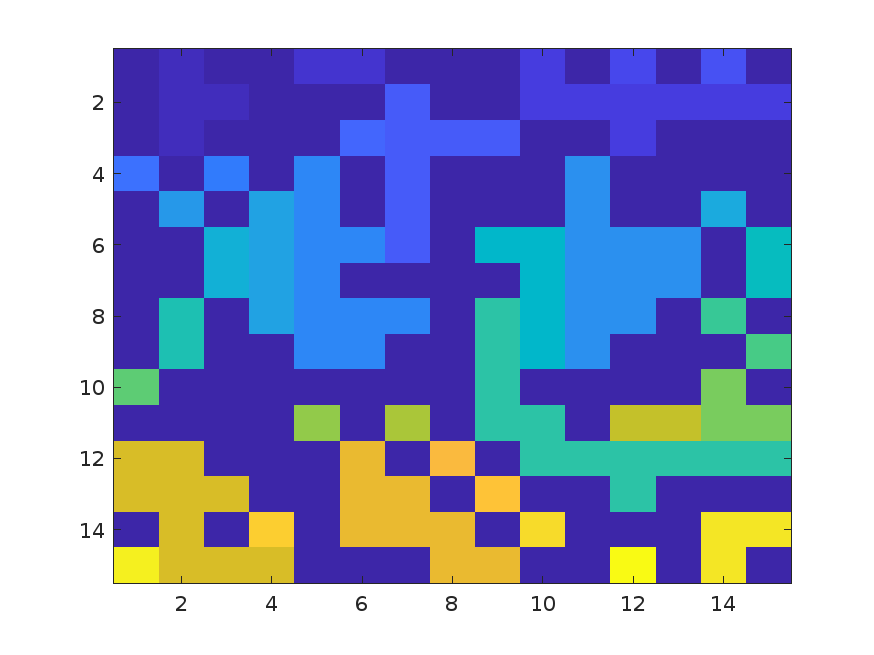
\includegraphics[width=\linewidth]{images/labels}
		
	\end{minipage}
	\caption{Esempio di etichettatura dei cluster con l’algoritmo di Hoshen-Kopelman}
	\label{fig:clustered}
\end{figure}
\noindent
Tuttavia, quando si incontra un caso come quello descritto nel punto \textbf{(4)}, occorre  memorizzare che i due cluster sono in realtà lo stesso. Questo viene fatto usando un vettore chiamato \textbf{Label of Label} (\texttt{LofL}), che contiene tutta l’informazione necessaria sulle label dei cluster. In particolare: 
\textbf{(1)} Per un \textit{good label}, viene memorizzata la taglia del cluster, mentre \textbf{(2)} per \textit{bad label} viene memorizzato il vero cluster a cui questa label appartiene.  Questa distinzione viene fatta attraverso i segni dei numeri interi contenuti in \texttt{LofL}. Ad esempio, i cluster associati al reticolo in Figura \ref{fig:basegrid} sono mostrati in Figura \ref{fig:clustered}, mentre di seguito è riportato il \texttt{LofL} corrispondete al reticolo preso in esame

\vspace{15px}
\noindent
\begin{tabular}{|c|*{12}{c|}}
	\hline
	\textbf{ID}   & 1 & 2 & 3 & 4 & 5 & 6 & 7 & 8 & 9 & 10 & 11 & 12 \\
	\hline
	\textbf{Val}  & 4 & 2 & 56 & -3 & -3 & 24 & -6 & 1 & 1 & -6 & -3 & 1 \\
	\hline
\end{tabular}

\vspace{10px}
\noindent
\begin{tabular}{|c|*{12}{c|}}
	\hline
	\textbf{ID}   & 13 & 14 & 15 & 16 & 17 & 18 & 19 & 20 & 21 & 22 & 23 & 24 \\
	\hline
	\textbf{Val}  & -10 & 1 & -10 & -3 & 2 & 2 & -3 & 1 & 1 & 1 & -3 & 1 \\
	\hline
\end{tabular}

\vspace{10px}
\noindent
\begin{tabular}{|c|*{11}{c|}}
	\hline
	\textbf{ID}   & 25 & 26 & 27 & 28 & 29 & 30 & 31 & 32 & 33 & 34 & 35 \\
	\hline
	\textbf{Val}  & 1 & -3 & 18 & -27 & 1 & 1 & -27 & -3 & -3 & -27 & -3 \\
	\hline
\end{tabular}

\vspace{15px}
\noindent
Tuttavia, sebbene l’algoritmo HK restituisca in modo corretto le taglie dei cluster, non garantisce che tutti i siti di un fissato cluster abbiano la stessa \texttt{label}. Per risolvere questo problema, possiamo effettuare una rietichettatura successiva. La Figura 3 ne mostra un esempio.

\begin{figure}[H]
	\centering
	\scriptsize % Riduce la dimensione del testo
	\setlength{\tabcolsep}{3.5pt} % Riduce lo spazio tra le colonne
	\renewcommand{\arraystretch}{1.3} % Riduce lo spazio verticale tra le righe
	\begin{minipage}{0.4\textwidth}
		\centering
		\begin{center}
			\begin{tabular}{|*{15}{c|}}
				\hline
				0 & 1 & 0 & 0 & 2 & 2 & 0 & 0 & 0 & 3 & 0 & 3 & 0 & 3 & 0 \\
				\hline
				0 & 1 & 1 & 0 & 0 & 0 & 6 & 0 & 0 & 3 & 3 & 3 & 3 & 3 & 3 \\
				\hline
				0 & 1 & 0 & 0 & 0 & 6 & 6 & 6 & 6 & 0 & 0 & 3 & 0 & 0 & 0 \\
				\hline
				8 & 0 & 9 & 0 & 6 & 0 & 6 & 0 & 0 & 0 & 3 & 3 & 0 & 0 & 0 \\
				\hline
				0 & 12 & 0 & 6 & 6 & 0 & 6 & 0 & 0 & 0 & 3 & 0 & 0 & 14 & 0 \\
				\hline
				0 & 0 & 6 & 6 & 6 & 6 & 6 & 0 & 3 & 3 & 3 & 3 & 3 & 0 & 17 \\
				\hline
				0 & 0 & 6 & 6 & 6 & 0 & 0 & 0 & 0 & 3 & 3 & 3 & 3 & 0 & 17 \\
				\hline
				0 & 18 & 0 & 6 & 6 & 6 & 6 & 0 & 3 & 3 & 3 & 3 & 0 & 20 & 0 \\
				\hline
				0 & 18 & 0 & 0 & 6 & 6 & 0 & 0 & 3 & 3 & 3 & 3 & 0 & 0 & 21 \\
				\hline
				22 & 0 & 0 & 0 & 0 & 0 & 0 & 0 & 3 & 0 & 0 & 0 & 0 & 3 & 0 \\
				\hline
				0 & 0 & 0 & 0 & 24 & 0 & 25 & 0 & 3 & 3 & 0 & 3 & 3 & 3 & 3 \\
				\hline
				27 & 27 & 0 & 0 & 0 & 27 & 0 & 29 & 0 & 3 & 3 & 3 & 3 & 3 & 3 \\
				\hline
				27 & 27 & 27 & 0 & 0 & 27 & 27 & 0 & 30 & 0 & 0 & 3 & 0 & 0 & 0 \\
				\hline
				0 & 27 & 0 & 27 & 27 & 27 & 27 & 27 & 0 & 3 & 3 & 3 & 0 & 3 & 3 \\
				\hline
				27 & 27 & 27 & 27 & 0 & 0 & 0 & 0 & 3 & 3 & 3 & 3 & 3 & 3 & 0 \\
				\hline
			\end{tabular}
		\end{center}
	\end{minipage}
	\hfill
	\begin{minipage}{0.45\textwidth}
		\centering
		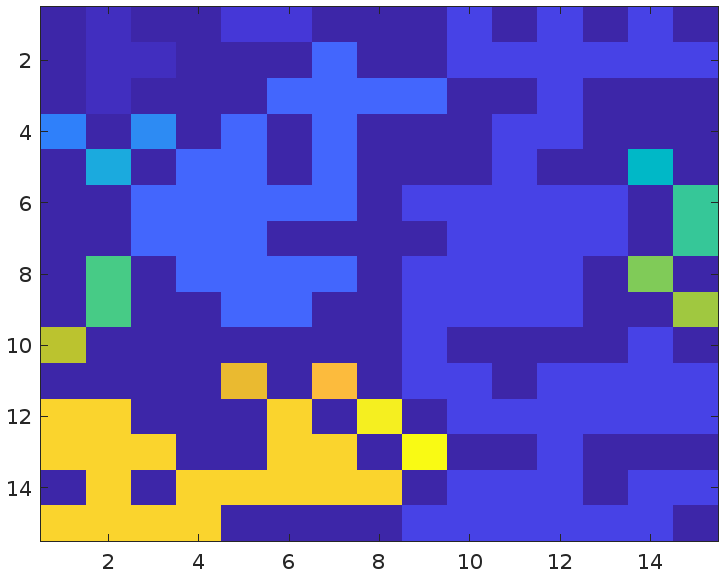
\includegraphics[width=\linewidth]{images/re-labelled}
	\end{minipage}
	\label{fig:relabelled}
	\caption{Esempio di rietichettatura dei cluster con etichette uniformi per ciascun gruppo}
\end{figure}
\noindent
A questo punto, l'obiettivo è determinare se esistono cluster percolanti all'interno del reticolo, ossia se esiste almeno un'etichetta condivisa tra la prima e l'ultima riga (percolazione verticale) o tra la prima e l'ultima colonna (percolazione orizzontale). Per fare ciò, possiamo sviluppare un algoritmo che, basandosi sull'estrazione delle etichette \textbf{uniche} presenti lungo i bordi della matrice, e mediante l'utilizzo dell'operazione \texttt{intersect},  verifichi l'esistenza di almeno una etichetta comune tra i bordi opposti. Se tale etichetta è presente, viene restituito \texttt{true} per il tipo di percolazione considerato, altrimenti \texttt{false}.
\\\\
\noindent
Si noti che, poiché ci interessa esclusivamente determinare il cluster di appartenenza della prima e dell’ultima riga e colonna per valutare la percolazione, è sufficiente rietichettare solo questi elementi, ignorando il centro del reticolo e risparmiando così tempo di calcolo. La Figura \ref{fig:relabelled-edge} ne mostra un esempio.
\begin{figure}
	\centering
	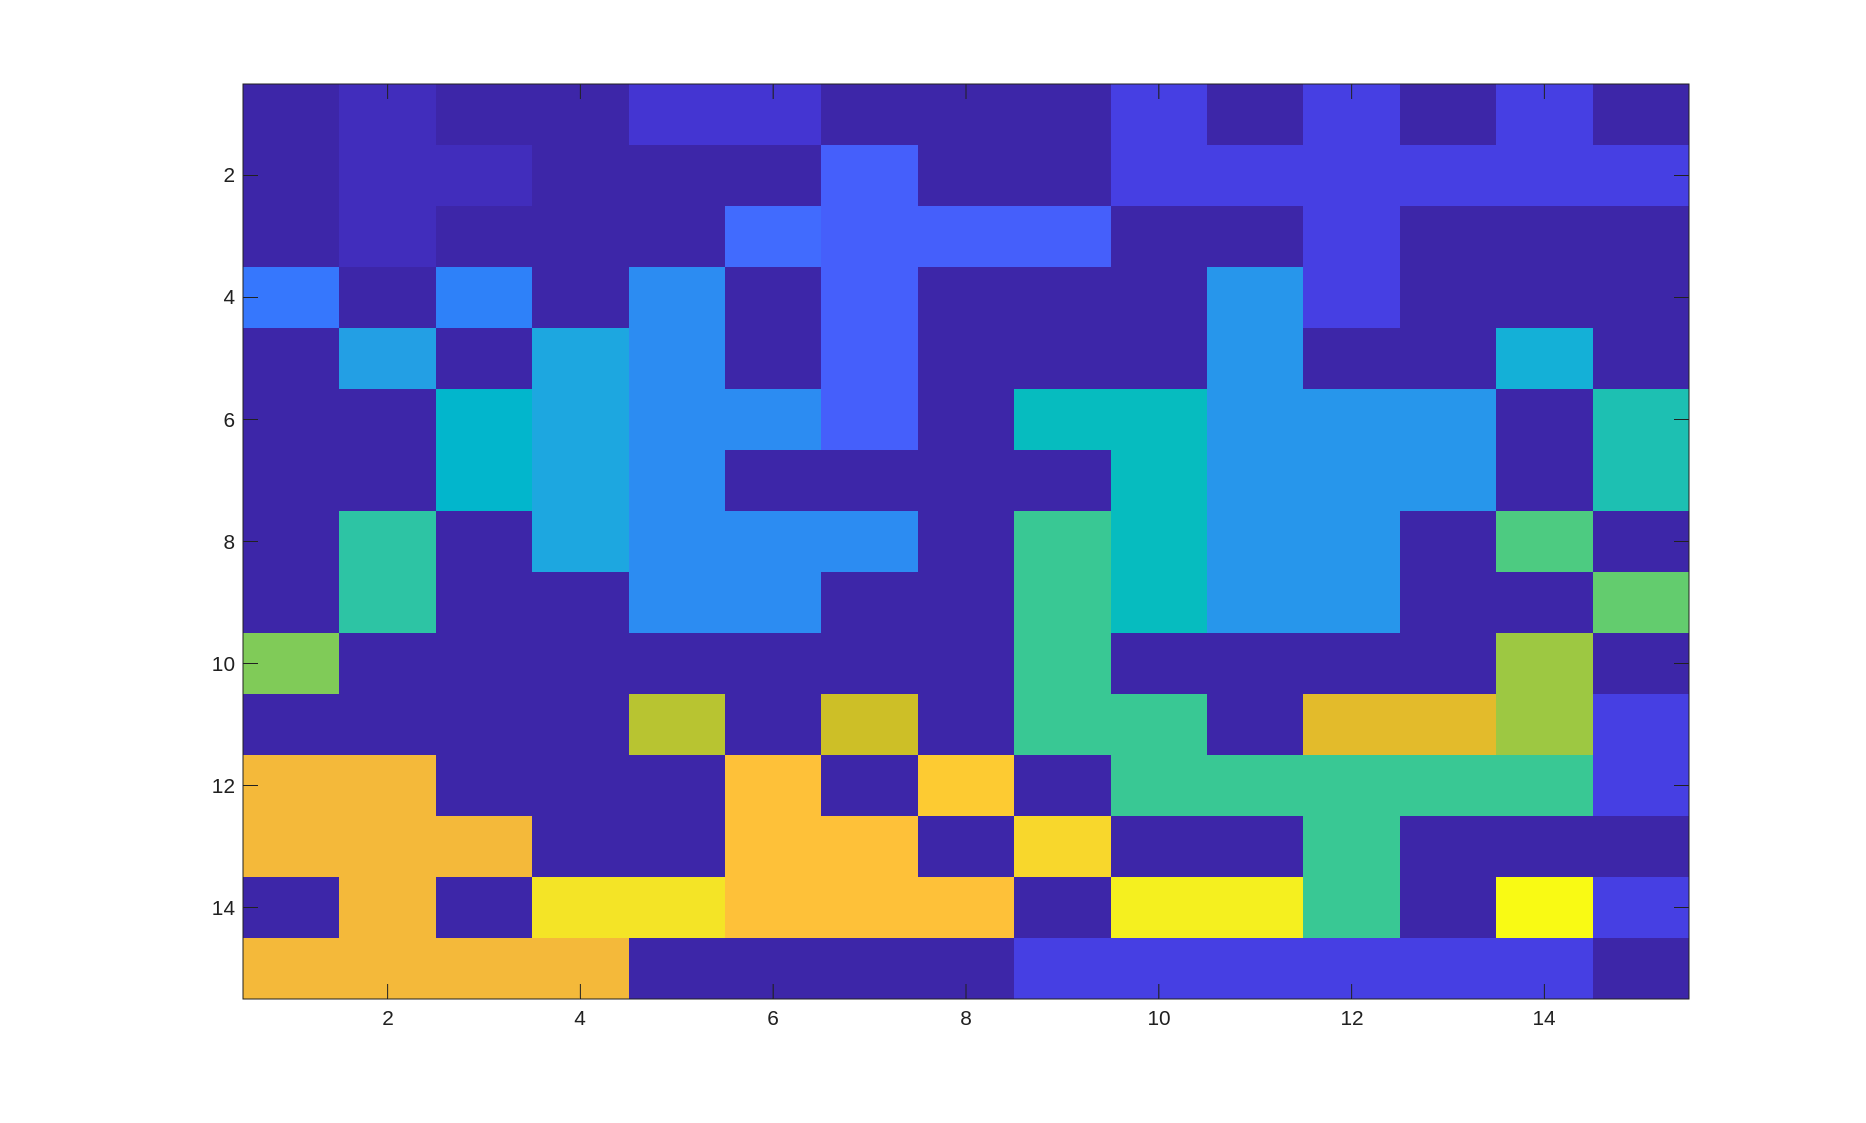
\includegraphics[width=0.7\linewidth]{images/re-labelled-edge}
	\caption{Esempio di rietichettatura dei soli bordi per il test di percolazione}
	\label{fig:relabelled-edge}
\end{figure}
\\\\
\noindent
Concludiamo dicendo che l'analisi della correttezza dell'implementazione proposta è stata effettuata non soltanto tramite test individuali sul singolo algoritmo, ma anche attraverso un confronto diretto con l'algoritmo naive presentato a lezione. Nello specifico, è stato generato un reticolo quadrato di taglia $100$, con una probabilità di colorazione dei siti pari al $60\%$. Tale reticolo è stato analizzato prima con l'algoritmo naive e successivamente con l'algoritmo HK76, confrontando i risultati ottenuti per la percolazione verticale e orizzontale. Questo confronto è stato ripetuto $10.000$ volte, e in tutti i casi i risultati forniti dai due algoritmi sono stati coincidenti. 
\\\\
\noindent
\textbf{Attenzione.} Di seguito sono riportate le principali funzioni matlab implementate. Il codice e i risultati ottenuti sono disponibili in versione integrale al link \textit{https://github.com/blkdmr/hk76}

\subsection*{hk76.m}
\begin{lstlisting}[style=matlabstyle]
function [TB, LR, LofL, labels] = hk76(mat)

    LofL = 0;

    N = size(mat,2);
    labels = zeros(N,N);
   
    lastLabel = 0;
    if mat(1,1) ~=0
        lastLabel = 1;
        labels(1,1) = lastLabel;
        LofL = hkclass(lastLabel, LofL, 0);
    end

    for i = 1:N % row
        for j = 1:N % cols
            
            if mat(i,j) ~= 0 % if site is colored
                badLabel = 0;

                % default case
                if i ~= 1 && j ~= 1 
                    left = labels(i,j-1);
                    up = labels(i-1, j);
                    

                    if left == 0 && up == 0 % no nearby clusters
                        lastLabel = lastLabel + 1;
                        nodeLabel = lastLabel;
                       
                    elseif left ~= 0 && up == 0 % left case
                        nodeLabel = left;

                    elseif left == 0 && up ~= 0 % up case
                        nodeLabel = up;
                        
                    elseif left ~= 0 && up ~= 0 && up == left % up and left case. NOT A BAD LABEL!
                         nodeLabel = left;

                    else % up and left case. BAD LABEL!
                        nodeLabel = min(up, left); 
                        badLabel = max(up, left);
                    end
                    LofL = hkclass(nodeLabel, LofL, badLabel);
                    labels(i,j) = nodeLabel;

                end
    
                if i == 1 && j ~= 1 % first row (only left case)
                    left = labels(i,j-1);
                    
                    if left == 0 
                        lastLabel = lastLabel + 1;
                        nodeLabel = lastLabel;
                    else
                        nodeLabel = left;
                    end

                    LofL = hkclass(nodeLabel, LofL, badLabel);
                    labels(i,j) = nodeLabel;
                end
                
                if i ~= 1 && j == 1 % first col (only up case)
    
                    up = labels(i-1, j);
    
                    if up == 0
                        lastLabel = lastLabel + 1;
                        nodeLabel = lastLabel;
                    else
                        nodeLabel = up;
                    end

                    LofL = hkclass(nodeLabel, LofL, badLabel);
                    labels(i,j) = nodeLabel;
                end
            end
        end
    end

    % Relabel first and last rows
    for i = 1:N
        if labels(1,i) ~= 0
            labels(1,i) = find_root(labels(1,i), LofL);
        end
        if labels(N,i) ~= 0
            labels(N,i) = find_root(labels(N,i), LofL);
        end
    end


    % Relabel first and last columns (excluding corners to avoid duplication)
    for i = 2:N-1
        if labels(i,1) ~= 0
            labels(i,1) = find_root(labels(i,1), LofL);
        end
        if labels(i,N) ~= 0
            labels(i,N) = find_root(labels(i,N), LofL);
        end
    end

    [TB, LR] = check_percolation(labels);

end
\end{lstlisting}

\subsection*{hkclass.m}
\begin{lstlisting}[style=matlabstyle]
function LofL = hkclass(nodeLabel, LofL, badLabel)
    
    % Make sure LofL can hold nodeLabel
    if numel(LofL) < nodeLabel
        LofL(nodeLabel) = 0;
    end

    if badLabel == 0
        % Find the true root of nodeLabel
        root = nodeLabel;
        while LofL(root) < 0
            root = -LofL(root);
        end
        % Count this site at the root
        LofL(root) = LofL(root) + 1;
    
    else
        % Find true roots of BOTH labels
        nodeRoot = find_root(nodeLabel, LofL);
        badRoot =find_root(badLabel, LofL);         
        
        % Are they already in the same cluster?
        if nodeRoot == badRoot
            % just add this site once
            LofL(nodeRoot) = LofL(nodeRoot) + 1;
        
        % Different clusters! merge badRoot under nodeRoot
        else
        
            % add full size of bad cluster, plus this new site
            LofL(nodeRoot) = LofL(nodeRoot) + LofL(badRoot) + 1;

            % make badRoot and badLabel both point to nodeRoot
            LofL(badRoot)  = -nodeRoot;
            LofL(badLabel) = -nodeRoot;
        end
    end
end
\end{lstlisting}

\subsection*{find\_root.m}
\begin{lstlisting}[style=matlabstyle]
function root = find_root(label, LofL)
	root = label;
	while LofL(root) < 0
		root = -LofL(root);
	end
end
\end{lstlisting}

\subsection*{check\_percolation.m}
\begin{lstlisting}[style=matlabstyle]
function [tbPercolates, lrPercolates] = check_percolation(labels)

    [N, ~] = size(labels);

    % Unique labels on top row
    topLabels    = unique(labels(1, :));
    topLabels(topLabels == 0) = [];  % remove 0 if any

    % Unique labels on bottom row
    bottomLabels = unique(labels(N, :));
    bottomLabels(bottomLabels == 0) = [];

    % Unique labels on left column
    leftLabels   = unique(labels(:, 1));
    leftLabels(leftLabels == 0) = [];

    % Unique labels on right column
    rightLabels  = unique(labels(:, end));
    rightLabels(rightLabels == 0) = [];

    % Check if any label is in both top and bottom
    if isempty(intersect(topLabels, bottomLabels))
        tbPercolates = false;
    else
        tbPercolates = true;
    end

    % Check if any label is in both left and right
    if isempty(intersect(leftLabels, rightLabels))
        lrPercolates = false;
    else
        lrPercolates = true;
    end
end
\end{lstlisting}
